% https://tex.stackexchange.com/a/746650/322482
\documentclass[tikz,border=5pt]{standalone}
\usepackage{amsmath}%
\renewcommand{\textuparrow}[1][black]{\textsuperscript{$\mathcolor{#1}{\uparrow}$}}%
\renewcommand{\textdownarrow}[1][black]{\textsuperscript{$\mathcolor{#1}{\downarrow}$}}%
\usetikzlibrary{arrows.meta}%
\begin{document}%
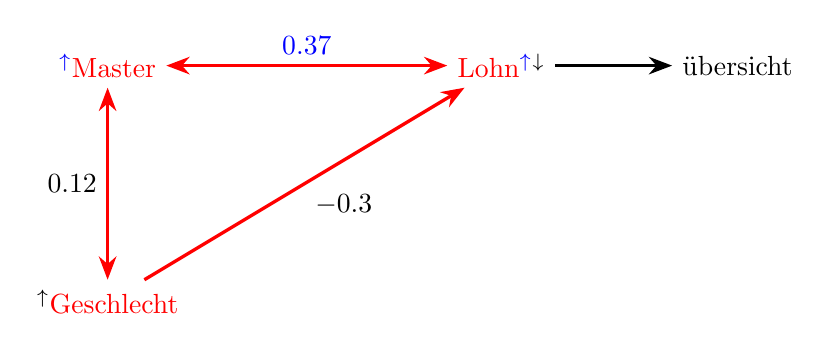
\begin{tikzpicture}[
        >={Stealth[red]},
        mynode/.style={rectangle,thick,text=red},
        every edge/.style={draw=red,very thick},
    ]
    \node[mynode] (EUR) at (5,3) {Lohn\textuparrow[blue]\textdownarrow};
    \node[mynode] (Master) at (0,3) {\textuparrow[blue]Master} 
                edge [<->] node[above,midway,font=\color{blue}] {$0.37$} (EUR);
    \node[mynode] (Frau) at (0,0) {\textuparrow Geschlecht} 
                edge [->] node[below right,midway] {$-0.3$}  (EUR)
                edge [<->] node[left,midway] {$0.12$}  (Master);
    \node[mynode,text=black] (obs) at (8,3) {übersicht}
                edge [<-,black,>={Stealth[black]}] (EUR);
\end{tikzpicture}
\end{document}